\documentclass[twocolumn]{amsart}
\usepackage[pdftex, a4paper, margin=0.7cm, nohead, nofoot]{geometry}
\usepackage[utopia]{mathdesign}
\usepackage{amsmath}
\usepackage{amsfonts}
\usepackage{bbm}
\usepackage{setspace}
\usepackage{scalefnt}
\usepackage{microtype}
\usepackage[absolute]{textpos}
\usepackage[compact]{titlesec}

\newcommand{\E}{\mathbb{E}}
\newcommand{\Cov}{\operatorname{Cov}}
\newcommand{\Var}{\operatorname{Var}}
\newcommand{\Exp}{\operatorname{Exp}}
\setlength{\parskip}{0pt}
\setlength{\parindent}{0pt}
\setlength{\TPHorizModule}{30mm}
\setlength{\TPVertModule}{\TPHorizModule}
\textblockorigin{10mm}{10mm} % start everything near the top-left corner
\titleformat{\section}{\centering\selectfont\bf}{}{0em}{}

\def\parsedate #1:20#2#3#4#5#6#7#8\empty{#6#7/#4#5/20#2#3\parsetime#8\empty}
\def\parsetime #1#2#3#4#5\empty{ #1#2:#3#4}
\def\moddate#1{\expandafter\parsedate\pdffilemoddate{#1}\empty}

% template taken from here: https://github.com/daleroberts/math-finance-cheat-sheet/

% More probability stuff
% https://wjgan.com/posts/latex.html
\usepackage{tikz}
\usetikzlibrary{calc,matrix}


\begin{document}
\pagestyle{empty}
\thispagestyle{empty}
\setstretch{0.8}
\scalefont{0.8}

\begin{center}
\textbf{MathStats}
\vskip0.2em
\end{center}

\section*{Densities}
\begin{equation*}
  f_{Y|X}(y|x) = \frac{f(x,y)}{f_{X}(x)} = \frac{f(x,y)}{\int_{-\infty}^{\infty}f(x,y)\,dy}
\end{equation*}
\begin{equation*}
  F_{Y|X}(y|x) = \int_{-\infty}^{y} \frac{f(x,v)}{f_{X}(x)}\,dv
\end{equation*}

\section*{Expectation}
\begin{equation*}
  \E[x^n] = \int_{-\infty}^{\infty} x^n f_{X}(x)
\end{equation*}
\begin{equation*}
  \E[Y] = \int_{-\infty}^{\infty}\E[Y|X=x]f_{X}(x)\,dx
\end{equation*}
\begin{equation*}
  \E[X^n] = \sum_{x:f(x)>0}x^{n}f(x)
\end{equation*}

\section*{Basics}

\begin{equation*}
  \Cov[X,Y] = \E[(X-\E[X])(Y-\E[Y])] = \E[XY] - \E[X]\E[Y]
\end{equation*}
\begin{equation*}
  \rho(X,Y) = \frac{\Cov[X,Y]}{\sqrt{\Var[X]\cdot\Var[Y]}} = \frac{\Cov[X,Y]}{\sqrt{\sigma_{X}\sigma_{Y}}}
\end{equation*}

\section*{Expectation Algebra}
\begin{equation*}
  \E[x^n] = \int_{-\infty}^{\infty} x^n f_{x}(x)
\end{equation*}

\section*{Variance Algebra}
\begin{equation*}
  \Var[X + Y] = \Var[X] + 2\Cov[X, Y] + \Var[Y]
\end{equation*}
\begin{equation*}
  \Var[X - Y] = \Var[X] - 2\Cov[X, Y] + \Var[Y]
\end{equation*}
\begin{equation*}
  \Var[XY] = \E[X^2] \cdot \E[Y^2] - {(\E[X] \cdot \E[Y])}^2
\end{equation*}
\begin{equation*}
  \Var[X/Y] = \Var[X \cdot (1/Y)] = \Var[(1/Y) \cdot X]
\end{equation*}
\begin{equation*}
  \Var[X] = \Cov(X, X) = E[X^2] - {E[X]}^2
\end{equation*}
\begin{equation*}
  \Var[aX+bY] = a^2\Var[X] + b^2 Var[Y] + 2ab\Cov[X,Y]
\end{equation*}

\section*{Jacobian}
\begin{equation*}
\mathbb{J}=\begin{vmatrix}
\frac{\partial x}{\partial u}\frac{\partial x}{\partial v} \\
\\
\frac{\partial y}{\partial u}\frac{\partial y}{\partial v} \\
\end{vmatrix}
\end{equation*}
\begin{equation*}
  \iint_{A}g(x,y)\,dx\,dy = \iint_{B}g(x(u,v),y(u,v))|J(u,v)|\,du\,dv
\end{equation*}

\section*{Calc}
\begin{equation*}
  \int u\,dv = uv-\int v\,du
\end{equation*}

\section*{Distributions}
Chi squared distribution with k=2 is a gamma/exp with the following params
\begin{equation*}
  \chi_{2}^{2} = \Gamma(\frac{1}{2},1) = \Exp(\frac{1}{2})
\end{equation*}
T Distribution
\begin{equation*}
  Z \sim \mathcal{N}(0, 1)
\end{equation*}
\begin{equation*}
  V \sim \chi_{k}^{2}
\end{equation*}
\begin{equation*}
  Z \perp V
\end{equation*}

% U SUBST

\section*{Linear Algebra}
\begin{center}
  Determinant

  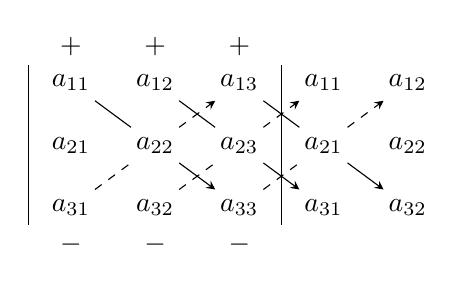
\begin{tikzpicture}[>=stealth]
    \matrix [%
    matrix of math nodes,
    column sep=1em,
    row sep=1em
    ] (sarrus) {%
      a_{11} & a_{12} & a_{13} & a_{11} & a_{12} \\
      a_{21} & a_{22} & a_{23} & a_{21} & a_{22} \\
      a_{31} & a_{32} & a_{33} & a_{31} & a_{32} \\
    };

    \path ($(sarrus-1-1.north west)-(0.5em,0)$) edge ($(sarrus-3-1.south west)-(0.5em,0)$)
    ($(sarrus-1-3.north east)+(0.5em,0)$) edge ($(sarrus-3-3.south east)+(0.5em,0)$)
    (sarrus-1-1)                          edge            (sarrus-2-2)
    (sarrus-2-2)                          edge[->]        (sarrus-3-3)
    (sarrus-1-2)                          edge            (sarrus-2-3)
    (sarrus-2-3)                          edge[->]        (sarrus-3-4)
    (sarrus-1-3)                          edge            (sarrus-2-4)
    (sarrus-2-4)                          edge[->]        (sarrus-3-5)
    (sarrus-3-1)                          edge[dashed]    (sarrus-2-2)
    (sarrus-2-2)                          edge[->,dashed] (sarrus-1-3)
    (sarrus-3-2)                          edge[dashed]    (sarrus-2-3)
    (sarrus-2-3)                          edge[->,dashed] (sarrus-1-4)
    (sarrus-3-3)                          edge[dashed]    (sarrus-2-4)
    (sarrus-2-4)                          edge[->,dashed] (sarrus-1-5);

    \foreach \c in {1,2,3} {\node[anchor=south] at (sarrus-1-\c.north) {$+$};};
    \foreach \c in {1,2,3} {\node[anchor=north] at (sarrus-3-\c.south) {$-$};};
  \end{tikzpicture}
\end{center}


\end{document}